%%%%%%%%%%%%%%%%%%%%%%%%%%%%%%%%%%%%%%% Titelseite
%\titlehead{
%\begin{center}
%\vspace{-2cm}
%
\includegraphics[scale=0.27]{Bilder/Otto.png} \\
%\end{center}
%}
\titlehead{
\vspace{-2cm}
\begin{center}
 
\includegraphics[scale=2]{Bilder/Otto_neu.eps}
\end{center}
\vspace{1cm}
}
\subject{\LARGE Masterarbeit\vspace{-5mm}}
\title{\huge Lighthouse Keeper \\ \LARGE Robotergestützte Erfassung und Evaluation \\ von iBeacon Konfigurationen\\
\vspace{1mm}
\textnormal{\small von}\vspace{-1cm}}
\author{\textnormal{\large André Pieper} \\[-3mm] \textnormal{\large Geb. 28.03.1988 in Berlin} \\[-3mm] \textnormal{\large Matrikelnummer: 184960} \vspace{0.5cm}}
\date{10. März 2015}
\publishers{
\begin{figure}[h]
$\begin{minipage}[b]{13cm}
	\vspace{0.5cm}
	\begin{normalsize}
	\begin{tabular}[h]{ll}
	Erstprüfer: & Jun.-Prof. Dr.-Ing. Sebastian Zug \\
	& Otto-von-Guericke-Universität \\
	& Fakultät für Informatik \\
	& Institut für Verteilte Systeme \\
	& Lehrstuhl Embedded Smart Systems \\
	& Universitätsplatz 2, D-39106, Magdeburg \\ \\

	Zweitprüfer: & Prof. Dr.-Ing. Abbas Omar \\
	& Otto-von-Guericke-Universität \\
	& Fakultät für Elektro- und Informationstechnik \\
	& Institut für Informations- und Kommunikationstechnik\\
	& Lehrstuhl für Hochfrequenz- und Kommunikationstechnik \\
	& Universitätsplatz 2, D-39106, Magdeburg \\ \\
	Betreuer: & Jun.-Prof. Dr.-Ing. Sebastian Zug 
	\end{tabular}
	\vspace{-2cm}
	\end{normalsize}
\end{minipage}
\begin{minipage}[b]{3cm}
\begin{flushright}
 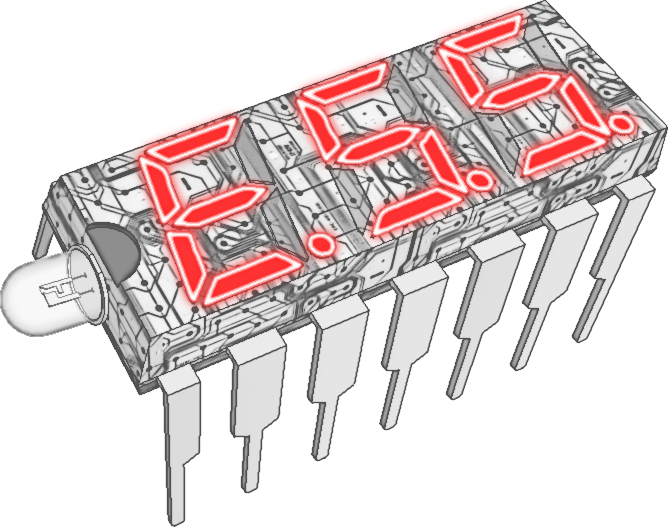
\includegraphics[scale=0.2]{Bilder/ESS.png} \\[2.5cm]
 
\includegraphics[scale=0.2]{Bilder/IIKT.png}
\end{flushright}
\end{minipage}$
\end{figure}
}

\begin{document}
\maketitle 
\newpage\thispagestyle{empty}~
\newpage
\setcounter{tocdepth}{2}

\section*{Kurzdarstellung}
Mit der Hilfe von mobilen Geräten ist es heutzutage möglich, die Position des Nutzers weltweit auf wenige Meter oder gar Zentimeter zu bestimmen. Jedoch verlieren sich die Signale der satellitengestützten Lokalisierungs-Systeme wie GPS, GLONASS und Galileo in Gebäuden, da sie durch deren Strukturen absorbiert, bzw. reflektiert werden. Durch diese Strukturen wird eine Lokalisierung innerhalb eines Gebäudes mithilfe von Funksignalen weitaus komplexer, als   


Hier steht dann das Vorwort. Hier stehen so Sachen wie, dass iBeacons die große Revolution in der Indoor-Lokalisierung sind. Dass sie in Flughäfen, Apple-Geschäften und (weitere Einsatzgebiete)... schon eingesetzt werden. Jedoch fehlt es an einer geeigneten Strategie die iBeacons zu verteilen (bisher wurde es abgeschätzt) und die Planung von Aufbau und Instandsetzumg von iBeacon-Lokalisierungsfeldern optimal umzusetzen. Denn in großen Gebieten, wie z.B. Einkaufshäuser, Lagerhallen und Flughäfen braucht man Hunderte von iBeacons, um die gesamte Fläche zu 100 Prozent abzudecken. Im Idealfall kann ich später in Matlab noch Gebiete einpflegen, an der die Karte nach Regionen aufgeteilt wird, in denen die Genauigkeit der Lokalisierung eingestellt werden kann. Damit ließe sich Robotergestützt ein Gebiet abfahren, in denen Vorschläge für die Positionierung von iBeacons anhand eines Optimierungsalgorithmusses generiert werden. Hierbei ließe sich wunderschön eine Pareto-Front bilden, die aus Anzahl von iBeacons und Genauigkeit pro Region Positionierungsvorschläge entwirft. Je nach Kundenwunsch. 